\section{文件系统}

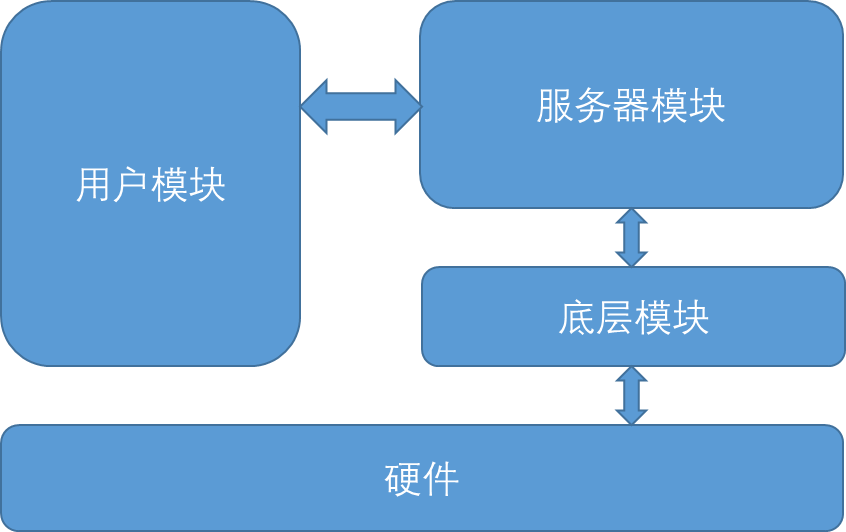
\includegraphics[width=6in]{figures/file/image107.png}

文件系统架构总体上分为3大模块,分别是用户模块,服务器模块,底层模块。

服务器模块负责打包底层模块文件读写函数,为外界提供统一的文件读写接口。

底层模块负责详细的页面划分,加载,缓存以及控制磁盘驱动。

用户模块与文件服务系统进程通信来进行文件读写活动。

\subsection{磁盘结构}

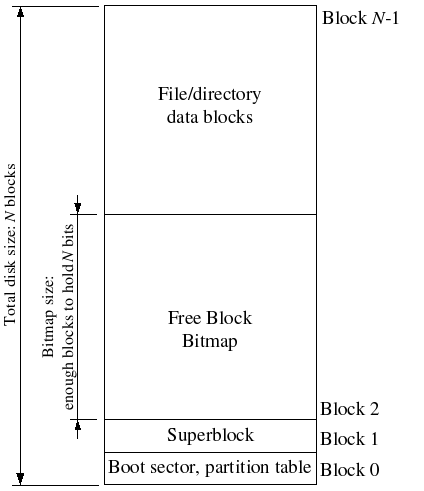
\includegraphics[width=6in]{figures/file/image108.png}

磁盘扇区大小512字节,而jos在此之上组织的块大小为4kB。与Linux不同的是此文件不使用inode,而是直接存储文件元数据,所以也不支持硬链接。

磁盘上文件结构是

\begin{itemize}
\item Block0 引导扇区,分区表
\item Block1 超级块
\item Block2~k Bitmap块,存储磁盘块占用信息
\item Blockk+1~N-1 数据块
\end{itemize}

\subsection{文件元数据}

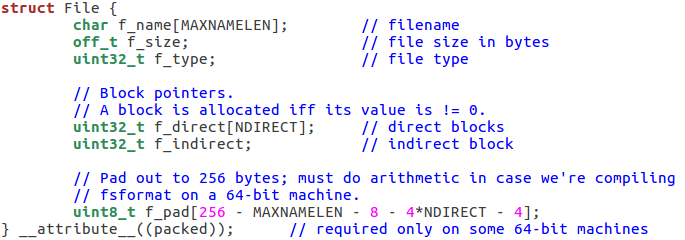
\includegraphics[width=6in]{figures/file/image109.png}

文件元数据使用file结构体存储,包含文件名,文件大小,10个直接块,一个间接块。文件的前10个block号会存在直接块里,其他的block会存在间接块指向的block里,可以额外存储4096/4=1024个文件块。

此文件系统不支持双重间接块和三重间接块,所以文件不能大于1034个文件块。

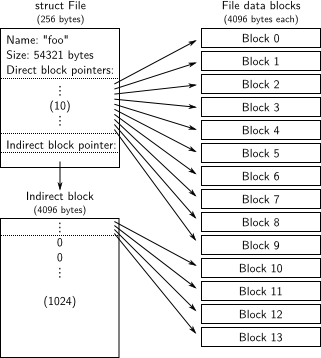
\includegraphics[width=6in]{figures/file/image110.png}

\subsection{目录与普通文件}

文件系统以相同的方式管理目录文件与普通文件,以f\_type区分,当文件块描述目录时,关联数据块内容为目录下的其他文件File数据块。

\subsection{块缓存}

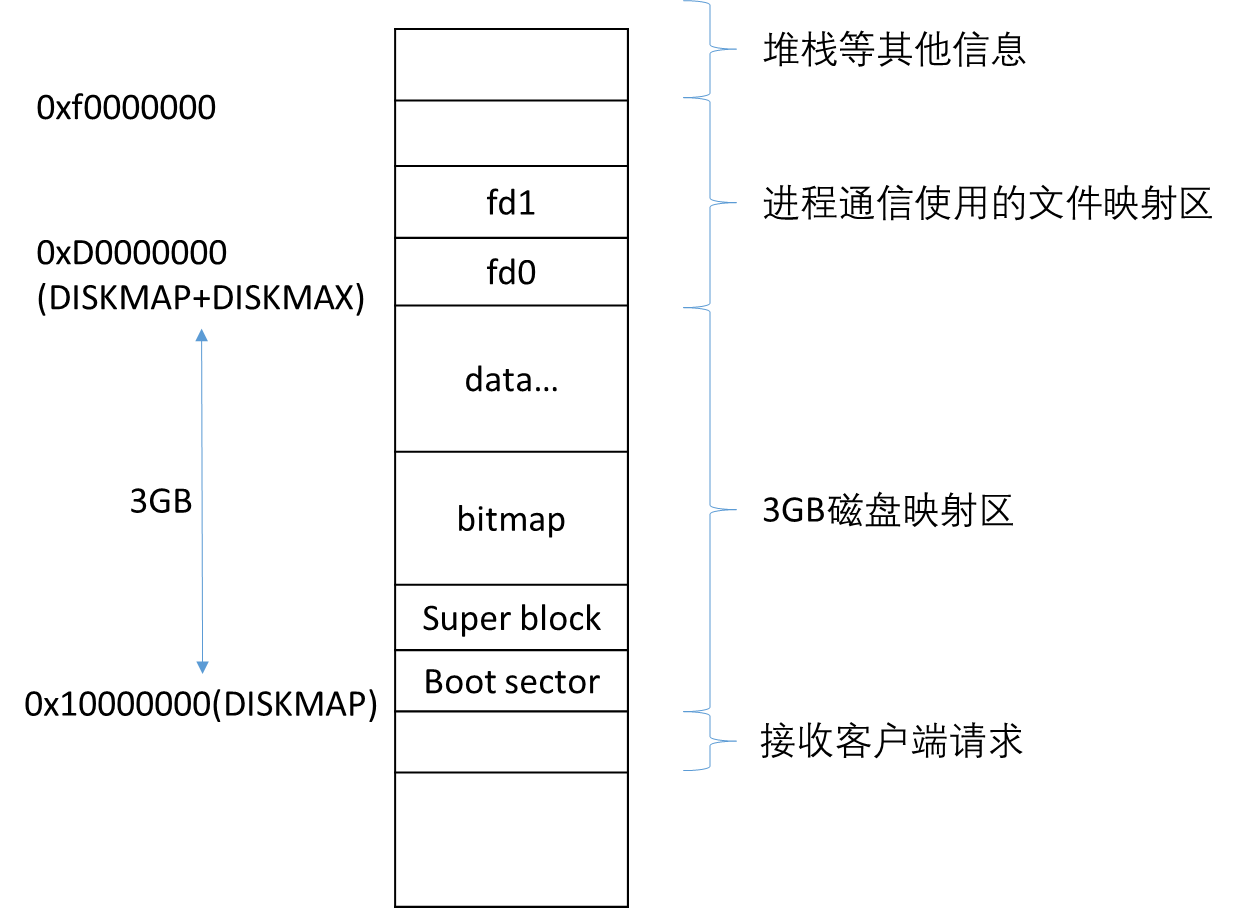
\includegraphics[width=6in]{figures/file/image111.png}

Jos中我们通过缓存技术来实现访问磁盘块。该机制可以支持最大3GB的磁盘。

我们将文件系统服务进程的虚拟地址空间(0x10000000 (DISKMAP)到0xD0000000 (DISKMAP+DISKMAX))对应到磁盘的地址空间(3GB)。

由于现代磁盘大于3GB,在32位机器上的真正的文件系统实现会很麻烦。这种缓冲区高速缓存管理方法在64位地址空间的机器上仍然是合理的。

映射方法:我们假装整个磁盘都已经被缓存到内存中,当我们想访问虚拟空间中的一个页时,由于虚拟空间还没有被映射,会发生页错误。在页错误处理程序中则会实际进行磁盘块到虚拟地址的映射并将该块磁盘内容缓存到内存中。

此时就可以恢复文件系统进程进行正常的文件访问。

Bc\_pgfault函数负责处理页面错误,处理的同时进行页面映射并从磁盘中缓存对应的块到内存中。

处理的步骤:

\begin{enumerate}
\item 根据地址计算出对应的blockno(块编号)
\item 检查地址范围是否超出(0x10000000 (DISKMAP)到0xD0000000 (DISKMAP+DISKMAX))的映射边界
\item 检查块编号是否超出块数
\item 将地址对齐到页起始位置
\item 页面映射
\item 调用ide\_read函数读取缓存块对应的数个磁盘页到内存中
\item 更新脏位
\end{enumerate}

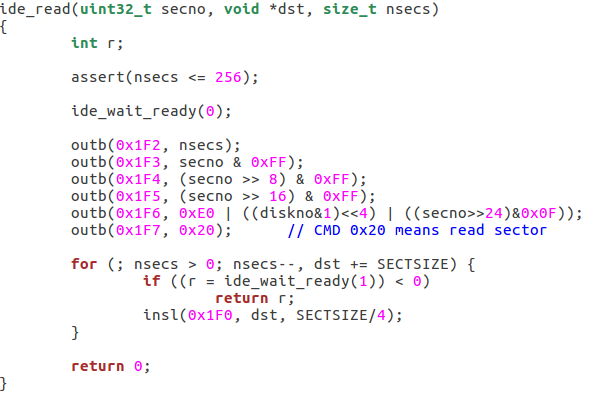
\includegraphics[width=6in]{figures/file/image112.png}

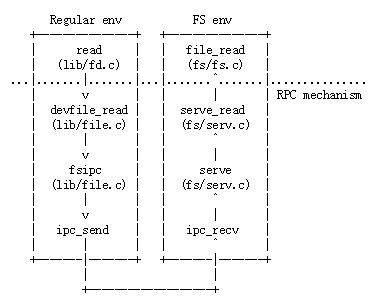
\includegraphics[width=6in]{figures/file/image113.png}


Flush\_block函数负责将缓存中的块写回到磁盘中。

处理步骤:

\begin{enumerate}
\item 根据地址计算出对应的blockno(块编号)
\item 检查地址范围是否超出(0x10000000 (DISKMAP)到0xD0000000 (DISKMAP+DISKMAX))的映射边界
\item 检查如果对应块没有映射就不写回
\item 检查如果对应块不是脏块(没有发生改动)就不写回
\item 最后将缓存写回到磁盘,检查是否成功并更新脏位
\end{enumerate}

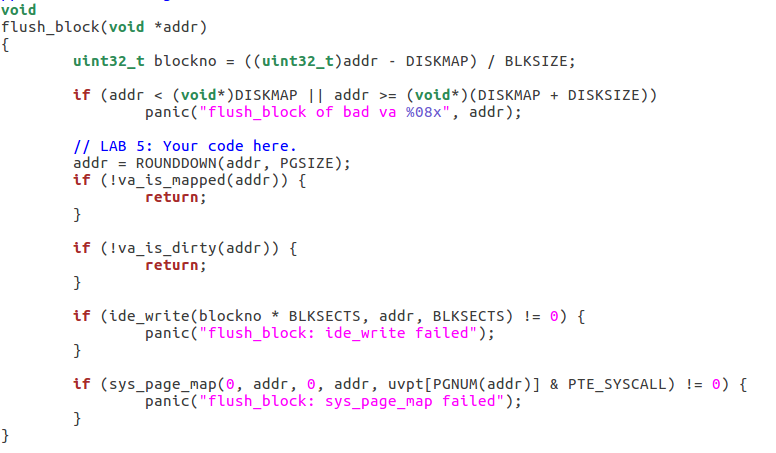
\includegraphics[width=6in]{figures/file/fig6.png}

\subsection{磁盘ide驱动文件}

Fs/ide.c中实现了ide\_read 和 ide\_write方法

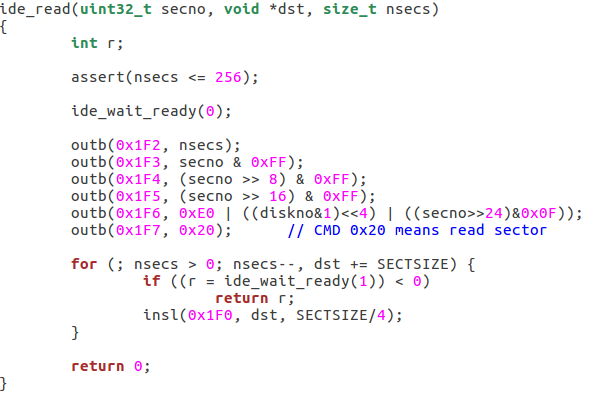
\includegraphics[width=6in]{figures/file/fig5.png}

\subsection{文件操作}

fs/fs.c中提供了各种函数 来实现您将需要解释和管理File结构,扫描和管理目录文件的条目,从根目录文件系统来解析绝对路径名。有一下几个主要函数:

\begin{itemize}
\item Walk\_path 完成目录解析
\item File\_block\_walk 找到一个文件的某一块
\item file\_get\_block 获取文件某一块
\item file\_read 读取某一个文件
\item file\_write 写入某一个文件
\end{itemize}

\subsection{文件系统服务器}

与启动引导时把文件读写作为系统调用不同,而是作为一个用户进程于是我们在创建文件读写进程时需要把I/O读写权限打开

文件服务器进程采用轮询的方式接收用户进程发送的文件读写请求,向用户进程返回信息

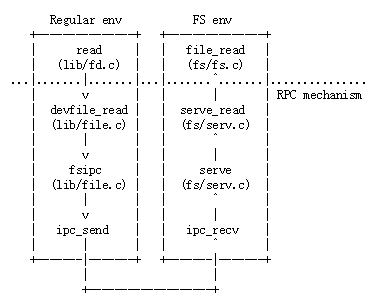
\includegraphics[width=6in]{figures/file/fig4.png}

虚线下面的所有内容都是从常规环境到文件系统环境的读取请求的机制。从头开始,read(我们提供的)在任何文件描述符上工作,并简单地调度到适当的设备读取功能,在这种情况下 devfile\_read(我们可以有更多的设备类型,如管道)。 devfile\_read 实现read专门针对磁盘上的文件。这个和lib / file.c中的其他devfile\_*函数 实现了FS操作的客户端,并且都以大致相同的方式工作,将请求结构中的参数捆绑在一起,调用 发送IPC请求,解包并返回结果。该fsipc 函数只是处理向服务器发送请求和接收答复的常见细节。

文件系统服务器代码可以在fs / serv.c中找到。它在serve函数中循环,无休止地通过IPC接收请求,将该请求分派给相应的处理函数,并通过IPC发回结果。在读取的例子中, serve将调度到serve\_read,将处理特定的IPC细节读取请求,如解开请求结构,最后调用 file\_read实际执行文件读取。

\subsection{用户使用的fd文件描述符}

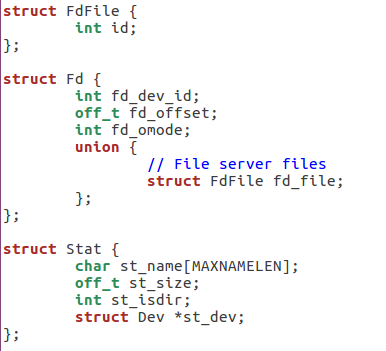
\includegraphics[width=6in]{figures/file/fig3.png}
